\chapter{绪论}

\section{研究背景与意义}

材料的组成、晶体结构与物性之间存在复杂的耦合关系。传统材料发现通常从经验规则、实验试错或给定结构的计算筛选出发：研究者先提出组成和结构，再通过实验表征或第一性原理计算判断其性质。这类流程能够提供可靠的物理依据，但候选空间随着元素种类、计量比、原子排布和晶胞自由度增加而迅速扩大。对每一个候选结构进行高精度电子结构计算，又会带来显著的计算成本。因此，如何在保证结构表示和评价可追溯的前提下减少无效候选，是计算材料设计中的重要问题。

机器学习推动了材料信息学从``结构到性质''的正向预测发展。给定组成、原子坐标和晶胞，模型可以近似预测形成能、能量高于凸包值、带隙、磁性或力学性质，从而加速高通量筛选。正向预测仍然需要一个已经给定的结构；当目标是寻找满足某种性质约束的新材料时，研究者还需要解决``从目标到结构''的逆向设计问题。逆向设计并不是正向函数的简单求逆，因为多个结构可能具有相近性质，模型误差和计算层级也会影响目标定义。生成式模型因此成为一种重要的候选产生机制：它从已知晶体分布中学习结构规律，再根据随机变量、组成或性质条件提出新的结构样本\citep{nouira2018,xie2022,jiao2023}。

晶体生成比一般的图像或文本生成具有更强的结构约束。一个候选晶体至少需要同时确定原子种类、周期分数坐标和晶胞；原子数和元素组合属于离散变量，坐标和晶胞参数属于连续变量；原子排序、整体平移、旋转以及周期复制还会造成表示等价。生成结果即使形式上可转换为结构文件，也可能存在过短原子间距、无效晶胞、异常能量或局部受力过大等问题。因而，材料逆向生成不能只以样本数量或形式新颖性作为目标，还必须同时考虑条件符合度、结构有效性、稳定性代理和局部几何一致性。

扩散模型为上述问题提供了一个适合多变量逐步生成的框架。相关方法可以在周期晶体图上建模坐标和晶胞，也可以进一步将元素种类纳入联合扩散。CDVAE 将变分表示与结构去噪结合，DiffCSP 在周期 \(E(3)\) 等变网络中联合生成晶格和原子坐标，MatterGen 则将原子种类、位置和晶胞作为相互耦合的字段，并支持面向化学体系、对称性和标量性质的条件生成\citep{xie2022,jiao2023,jiao2024,zeni2025}。这些模型提高了候选生成的自动化程度，但推理过程仍然存在两个与本文直接相关的问题。

第一个问题是条件属性控制。分类器无关引导通过条件得分与无条件得分的差异增强目标条件，是扩散模型中常用的推理阶段机制\citep{ho2020,song2021,ho2022}。固定引导强度具有实现简单、额外训练成本低的优点，但不同样本、不同扩散阶段和不同字段的条件响应可能并不相同。对所有样本采用同一强度，可能无法充分利用少量有利的条件偏离；直接根据中间残差在线调整，又可能把不稳定信号放大到结构质量。本文因此研究如何在有限推理预算内保留可靠基线、展开少量候选并依据终点代理约束作出选择。

第二个问题是局部结构物理一致性。机器学习原子间势可以低成本估计能量、力和应力，已广泛用于结构筛选、松弛和材料搜索\citep{merchant2023,chen2022,batzner2022,batatia2022,deng2023,yang2024mattersim}；但在许多生成流程中，神经势主要用于生成完成后的评价或优化。若在扩散过程早期直接对高噪声状态计算力，力的排序和方向可能不可靠；若完全等到终态再处理，又无法研究外部物理反馈如何影响生成轨迹。本文围绕这一时间接口，先校准预测干净结构在后期阶段的可靠性，再研究神经势原子力进入逆扩散位置更新的方式。

本文以 MatterGen 作为冻结的基础生成模型，研究对象是其推理阶段的条件引导与神经力场反馈，而不是重新提出或重新训练 MatterGen。两个研究问题分别对应条件属性控制和代理局部结构一致性，评价时使用配对种子、预注册指标以及 Matter\allowbreak Sim 和 CHGNet 代理模型，并明确保留无 DFT 验证这一证据边界。这样的研究具有两方面意义：在方法层面，考察生成模型内部得分、终点评价和外部物理代理之间如何形成可审计的推理接口；在应用层面，为不同目标优先级下的候选生成和局部结构筛选提供可复现的实验依据。

从计算机专业硕士论文的角度看，本文关注的不是单一模型在某个数据集上的分数，而是一个包含状态管理、推理控制和证据审计的生成系统。参考轨迹需要同时保存采样器状态与随机数状态，候选选择需要把计算预算写入算法定义，神经力反馈需要处理坐标系、时间阶段和异常路径，最终结论还要通过匹配种子和跨代理评价检验。这些环节把生成模型、图神经网络、数值采样和实验设计连接起来，形成可实现、可复现和可分析的计算机技术问题。

\section{国内外研究现状}

\subsection{材料逆向设计与生成式材料设计}

材料逆向设计通常将目标性质、组成范围或结构约束作为输入，输出一个或多个候选材料。早期方法常将生成建模与潜空间优化结合，在连续潜变量中寻找具有较低形成能或目标属性的结构。CrystalGAN 将生成对抗网络用于晶体结构学习，并通过潜空间或生成结果筛选探索新的化学组合\citep{nouira2018}；后续的可逆晶体表示工作则将结构编码为可生成的字符串或图结构，使性质条件可以与序列模型结合\citep{xiao2023}。这些方法说明，表示方式会直接影响模型能否恢复有效晶胞、周期邻接和元素关系。

另一条路线是高通量预测与搜索。GNoME 通过大规模图模型和主动学习流程扩展稳定晶体候选，再使用更高成本的计算和实验流程进行后续筛选\citep{merchant2023}。这类工作展示了机器学习在扩大候选覆盖范围方面的能力，同时也说明``预测稳定''与``可以合成、具有目标功能''之间仍需多层验证。生成模型的作用更接近提出结构候选和改善搜索起点，不能替代第一性原理、实验表征或工艺验证。

随着逆向设计任务从单一组成搜索扩展到复杂目标属性，研究重点逐渐转向可控生成。条件变分模型可以把组成、压力或材料属性输入解码器；扩散模型可以通过条件得分、结构约束或外部预测器改变采样分布；自回归模型则可以直接以 CIF 或结构字符串为序列进行生成。近期综述把表示、生成架构和属性约束视为生成式材料设计的三个核心环节，并指出数据兼容性、计算资源和有效生成率仍然是共性挑战\citep{long2024}。本文选取 MatterGen 作为实验基础，正是因为它在同一扩散框架中联合处理元素、位置和晶胞，并支持属性条件。

\subsection{晶体材料生成模型的发展}

晶体生成模型的发展可以按生成表示和建模方式粗略分为三类。第一类以体素、图或潜变量为基础，利用 VAE、GAN 或其他潜空间模型学习结构分布。CrystalGAN 代表了较早将 GAN 用于晶体结构生成的尝试\citep{nouira2018}；CDVAE 则将周期图编码器、属性预测器和扩散解码器结合起来，在结构重建、有效生成和属性优化任务上进行统一评估\citep{xie2022}。这些工作把周期边界和几何对称性纳入模型设计，但对变原子数、复杂晶胞和跨化学体系生成的处理方式仍各不相同。

第二类是等变扩散模型。DiffCSP 使用周期 \(E(3)\) 等变去噪网络，并在分数坐标中联合更新晶格和原子位置，主要面向给定组成的晶体结构预测，也扩展到从头晶体生成\citep{jiao2023}。DiffCSP++进一步把空间群约束转化为晶格对数空间和 Wyckoff 位置约束，支持具有空间群条件的可控生成\citep{jiao2024}。UniMat 采用可扩展的材料生成扩散框架，面向更大规模和更复杂的化学系统，研究了条件生成与稳定候选发现\citep{yang2024}。这些方法体现了周期性、旋转等变性和晶胞生成在晶体扩散中的核心地位。

第三类是序列和语言模型。SLICES 将晶体拓扑与组成编码为可逆字符串，并用循环神经网络生成满足目标性质的候选结构\citep{xiao2023}。CrystaLLM 直接对标准化 CIF 文本进行自回归建模，并根据组成或空间群提示生成结构文件\citep{antunes2024}。序列模型便于使用成熟的语言建模和搜索算法，但生成结果需要经过 CIF 解析、周期结构重建和物理评价；文本合法并不自动意味着晶体几何有效。

MatterGen 位于上述发展线索的交汇处。它采用面向无机晶体的联合扩散框架，对原子种类、周期坐标和晶胞进行字段特定的噪声建模，并通过条件适配支持属性引导\citep{zeni2025}。与主要接受固定组成的 CSP 方法相比，MatterGen 更适合作为本文的基础生成器；与只在终点进行结构优化的流程相比，它为研究采样期间的推理接口提供了完整的反向轨迹。本文的工作建立在这个基础模型之上，不改变其权重和基本字段定义。


            \begin{longtable}[]{@{}
  >{\raggedright\arraybackslash}p{(\linewidth - 10\tabcolsep) * \real{0.1667}}
  >{\raggedright\arraybackslash}p{(\linewidth - 10\tabcolsep) * \real{0.1667}}
  >{\raggedright\arraybackslash}p{(\linewidth - 10\tabcolsep) * \real{0.1667}}
  >{\raggedright\arraybackslash}p{(\linewidth - 10\tabcolsep) * \real{0.1667}}
  >{\raggedright\arraybackslash}p{(\linewidth - 10\tabcolsep) * \real{0.1667}}
  >{\raggedright\arraybackslash}p{(\linewidth - 10\tabcolsep) * \real{0.1667}}@{}}\bicaption{代表性晶体生成方法对比}{Comparison of Representative Crystal Generation Methods}\label{tab:1-1}\\

        \toprule
        \noalign{}
\begin{minipage}[b]{\linewidth}\raggedright
方法
\end{minipage} & \begin{minipage}[b]{\linewidth}\raggedright
主要范式
\end{minipage} & \begin{minipage}[b]{\linewidth}\raggedright
组成处理
\end{minipage} & \begin{minipage}[b]{\linewidth}\raggedright
位置与晶胞
\end{minipage} & \begin{minipage}[b]{\linewidth}\raggedright
条件控制
\end{minipage} & \begin{minipage}[b]{\linewidth}\raggedright
生成期物理反馈
\end{minipage} \\
\midrule\noalign{}
\endfirsthead
        \toprule
        \noalign{}
\begin{minipage}[b]{\linewidth}\raggedright
方法
\end{minipage} & \begin{minipage}[b]{\linewidth}\raggedright
主要范式
\end{minipage} & \begin{minipage}[b]{\linewidth}\raggedright
组成处理
\end{minipage} & \begin{minipage}[b]{\linewidth}\raggedright
位置与晶胞
\end{minipage} & \begin{minipage}[b]{\linewidth}\raggedright
条件控制
\end{minipage} & \begin{minipage}[b]{\linewidth}\raggedright
生成期物理反馈
\end{minipage} \\
\midrule\noalign{}
\endhead


\bottomrule\noalign{}
\endlastfoot
CrystalGAN \citep{nouira2018} & GAN & 潜空间或生成约束 & 结构表示相关 & 潜空间/后处理 & 无在线力反馈 \\
CDVAE \citep{xie2022} & VAE+扩散 & 潜变量预测 & 周期坐标与晶胞 & 属性优化 & 结构稳定先验 \\
DiffCSP \citep{jiao2023} & 周期等变扩散 & 通常给定组成 & 联合生成晶格与坐标 & 组成或任务条件 & 无在线力反馈 \\
DiffCSP++ \citep{jiao2024} & 约束扩散 & 给定或受约束 & 空间群与 Wyckoff 约束 & 空间群条件 & 结构约束 \\
UniMat \citep{yang2024} & 可扩展扩散 & 条件生成 & 晶体结构 & 组成/数据条件 & 无在线力反馈 \\
SLICES \citep{xiao2023} & 自回归字符串 & 字符串编码 & 解码后重建 & 目标属性 & 后续松弛 \\
CrystaLLM \citep{antunes2024} & CIF 自回归模型 & 提示或给定 & CIF 文本 & 组成/空间群提示 & 后处理评价 \\
MatterGen \citep{zeni2025} & 三字段联合扩散 & 联合生成 & 位置与晶胞联合生成 & 化学、对称性、标量属性 & 本文冻结基线 \\
SCIGEN \citep{okabe2025} & 结构约束扩散 & 约束生成 & 几何图案条件 & 蜂窝、kagome等结构 & 结构先验 \\
PODGen \citep{ye2026} & 预测器引导 MCMC & 通用生成器 & 生成结构 & 多属性预测器 & 预测器引导采样 \\
\end{longtable}
表1-1用于定位技术路线，不用于直接比较不同论文的数值结果。各方法使用的数据集、结构表示、训练规模和评价协议不同；本文只提取与研究问题有关的生成对象、条件接口和物理反馈方式。

\subsection{扩散模型在晶体生成中的应用}

扩散模型的优势在于可以把复杂结构分布分解为多个噪声阶段的去噪任务。对晶体而言，噪声过程不能简单复制图像领域的各向同性高斯扰动：分数坐标具有周期性，晶胞属于矩阵变量，原子种类属于离散类别，三者还通过局部邻域耦合。CDVAE 通过结构扩散解码器处理周期材料；DiffCSP 使用周期等变网络；MatterGen 则进一步将原子类型加入三字段联合生成\citep{xie2022,jiao2023,zeni2025}。

条件方式也呈现多样化。DiffCSP++把空间群约束纳入扩散过程，SCIGEN在扩散步骤中注入蜂窝、kagome等几何结构先验，以产生具有特定结构图案的候选\citep{jiao2024,okabe2025}。这些方法表明，条件可以作用于组成、对称性、几何结构或属性目标，而不一定只由网络输入端的标签完成。对本文而言，这些工作提供了一个重要背景：推理时改变采样轨迹已经成为材料生成的重要研究方向，但不同方法的约束对象、计算预算和安全判据并不相同。

2025---2026年的工作进一步关注目标导向生成。MatterGen展示了面向多种化学和标量条件的基础生成能力\citep{zeni2025}；PODGen把多个性质预测器与生成模型结合，通过 MCMC 采样调整生成分布，并用于拓扑材料的目标搜索\citep{ye2026}。SCIGEN和PODGen都说明外部约束或预测模型可以在生成过程中改变候选分布，但它们与本文的研究接口不同：本文在冻结的 MatterGen 上保存精确 C0 参考轨迹，在有限候选预算下进行终点接受与回退；另一路则把经阶段校准的神经势原子力注入后期 position predictor。本文据此把贡献限定为两个具体的推理阶段方法，而不把一般的条件生成或约束采样重新命名为本文创新。

\subsection{条件属性控制与引导生成}

条件生成的目标是让样本分布同时满足结构先验和目标属性。常见实现包括在训练阶段把条件嵌入输入生成器、使用外部分类器或预测器提供梯度、采用分类器无关引导，以及在生成后进行候选筛选。分类器无关引导以同一网络产生条件和空条件预测，再按引导强度组合两者\citep{ho2022}。它避免了单独训练分类器的接口成本，因此适合 MatterGen 这类已有条件适配模块的模型。

固定 CFG 强度的优点是规则清楚、运行成本可预测、容易进行配对比较。其局限在于，条件得分差异会随样本、字段和噪声阶段变化；一个适合某个阶段的强度不一定适合另一个阶段。PODGen从外部预测器和 MCMC 角度调整采样分布，SCIGEN则从结构约束角度改变去噪轨迹\citep{okabe2025,ye2026}。这些方向与本文关注的问题相近，但并不直接回答``在冻结 MatterGen 中，如何以有限额外预算保留一条可精确恢复的 C0 参考轨迹，并对候选终点实施安全回退''。

本文前期对多字段残差驱动的在线 Adaptive CFG 进行了机制分析。结果显示，反事实候选中存在可利用的属性改善空间，但简单在线控制在新样本上缺乏稳定复现；学习型 Linear-K2 也没有在相同预算下确认优于固定策略。因此，最终问题被重新表述为参考保留、有限分支和终点验证，而不是把 Adaptive CFG 作为最终创新名称。这一表述与文献中的条件采样研究相容，同时避免把探索性控制器的失败过程包装成已验证方法。

\subsection{神经网络原子间势与生成结构优化}

神经网络原子间势（MLIP）学习结构与能量、力或应力之间的映射，以较低推理成本近似某一计算层级。M3GNet采用包含三体相互作用的图网络，在较广元素范围内预测材料能量和力\citep{chen2022}；NequIP通过 \(E(3)\) 等变特征提高数据效率和几何一致性\citep{batzner2022}；MACE将高阶等变消息传递与原子簇展开结合，用于快速力场建模\citep{batatia2022}。CHGNet在晶体图中引入电荷和磁矩相关信息，提供能量、力、应力和磁矩等预测\citep{deng2023}；Matter\allowbreak Sim则面向广元素、温度和压力范围，原生输出能量、原子力和应力\citep{yang2024mattersim}。

在材料发现流程中，MLIP通常承担三个角色。第一，用于在大规模候选中快速估计能量或稳定性，减少昂贵计算调用；第二，作为结构松弛器，把生成候选推向当前代理势下的局部低能区域；第三，作为独立或交叉评价器，比较不同生成方法的局部受力、能量和结构偏移。GNoME的工作也体现了机器学习势与大规模结构搜索、稳定性筛选结合的价值\citep{merchant2023}。但是，代理力较小只说明结构在所用势面上的局部一阶残差较小，不能直接等价于热力学稳定、实验可合成或 DFT 结论。

现有生成---评价流程多在终点调用 MLIP，或者把 MLIP 用作生成后的连续松弛器。相邻领域已经出现将力信息用于扩散采样的研究，例如 ConfDiff 将力引导思想用于蛋白质构象生成\citep{wang2024}；这说明``外部物理方向进入扩散轨迹''具有一般方法背景，但蛋白质构象、无机晶体周期坐标和 MatterGen 三字段采样并不是同一问题。对无机晶体而言，神经势面对的是周期晶胞、分数坐标和元素组合，过早使用含噪结构进行力评价还可能引入不可靠反馈。

因此，本文第二条研究路线关注一个更窄的接口：先用预测干净结构与最终 MaxF 的阶段排序相关性确定可用的后期窗口，再将 Matter\allowbreak Sim 笛卡尔力映射为周期分数坐标修正，并通过 predictor 的实际 score 系数注入位置更新。CHGNet不参与在线反馈，用作跨势独立代理评估器。研究目标是检验生成期代理局部结构一致性是否改善，证据边界仍限定于冻结 MLIP 代理，且 DFT\_VERIFIED=false。

\subsection{现有研究的主要不足}

综合上述研究，可以把与本文相关的不足归纳为两个相互独立的问题。

第一，条件晶体生成已经能够接收组成、空间群或属性条件，但固定强度引导缺少样本和轨迹层面的推理时选择机制；外部预测器或约束采样虽然提供了其他方向，却不一定同时保存一条可复现的参考轨迹，也不一定设置与结构质量绑定的回退。对冻结 MatterGen 而言，需要一种明确限制候选数量、控制额外 score 调用、使用终点代理约束并在失败时返回 C0 的推理方案。

第二，神经势已经能够快速评价和松弛晶体，但生成模型与神经力场之间的在线接口仍有阶段可靠性和坐标变换问题。含噪结构不一定适合直接计算原子力；笛卡尔力也不能未经变换直接加到分数坐标上；没有幅度控制和异常回退时，外部反馈可能破坏周期几何或属性条件。因而需要在后期可靠窗口内进行有限、可审计的力反馈实验。

本文不把上述不足写成对全部现有方法的否定，也不声称两个方法在文献中没有任何相近思想。研究空白限定在当前实验对象和接口：在冻结 MatterGen 上，参考轨迹保留的有限多分支条件引导与安全回退；以及阶段可靠性校准的后期神经力场反馈。后续章节将分别给出两条路线的实现、确认实验和证据边界。

为了使研究问题可被计算机实验检验，本文进一步把``改进''拆成可观察的接口行为。属性路线要求候选必须从同一保存状态继续运行，候选数量和 score 调用量在实验前冻结，终点选择必须记录接受或回退原因；局部结构路线要求每次神经势调用对应明确的扩散阶段，力向量经坐标映射和幅度限制后才能进入位置更新，并保留异常时的原始 score。这样的定义把方法差异落实为状态、预算、坐标和分支决策，便于在相同种子下复现，而不是只依赖一次生成结果的事后解释。

在证据解释上，本文把代理模型当作有适用范围的计算工具。Property MAE、E-hull、Stable、Validity、MaxF、Mean Force 和 RMSD 分别描述条件误差、能量相对位置、几何与评价可用性以及局部受力或松弛偏移；它们不能被压缩成未经注册的综合分数。配对差异、置信区间、胜平负和跨代理方向共同决定结论强度，任何外部任务、不同 checkpoint 或真实实验结论都需要重新建立数据和验证流程。

\section{本文研究内容}

本文围绕无机晶体逆向生成中的条件属性控制和代理局部结构一致性开展研究，基础模型采用冻结的 MatterGen，研究阶段不重新训练主干权重。全文研究内容分为三个层次。

第一，分析 MatterGen 条件生成的推理机制。本文从固定 CFG 出发，拆分原子种类、位置和晶胞三个字段的条件---无条件得分残差，考察不同阶段、不同字段和不同样本的引导差异；随后通过反事实 Oracle、风险校准和字段归因实验判断潜在的候选改善空间及在线控制风险。这部分工作的作用是确定问题结构，为最终方法选择提供机制证据，不把探索性 Adaptive CFG 当作最终贡献。

第二，提出参考轨迹保留的预算约束多分支条件引导与安全回退方法。该方法在 C0 的共享前缀后保存完整采样状态和随机数状态，按冻结的候选库展开固定双候选分支；候选完成后，使用属性误差、Validity、Stable和 E-hull等冻结代理约束进行终点选择。只有严格改善属性且通过质量条件的候选才被接受，否则返回可精确复现的 C0。最终确认策略为 Fixed-K2。学习型 Linear-K2作为负消融保留，用于说明当前特征和样本规模下的样本级候选分配没有得到独立支持。

第三，提出基于阶段可靠性校准的后期神经力场引导扩散方法 RC-NFGD。该方法先比较多个扩散阶段的预测干净结构 MaxF 与最终结构 MaxF 的排序一致性，冻结后期介入窗口；然后调用 Matter\allowbreak Sim计算原子力，将去平移、归一化和有界的笛卡尔力位移转换为分数坐标修正，并补偿 position predictor 的 score 系数。原子类型、晶胞和 corrector保持 MatterGen原有更新，异常情况执行安全回退；Formal256使用CHGNet作为未参与在线力反馈的独立代理评估器。

上述研究内容对应两类不同目标。Fixed-K2主要改善目标属性条件的终点准确性，代价是增加约2.2倍 MatterGen score调用；RC-NFGD主要改善神经势代理下的局部受力和松弛位移，Property MAE存在轻微代价。两者都通过配对种子和冻结指标进行评价，但当前联合兼容实验未支持协同增益，因此论文分别报告两项创新。


            \begin{longtable}[]{@{}
  >{\raggedright\arraybackslash}p{(\linewidth - 6\tabcolsep) * \real{0.2500}}
  >{\raggedright\arraybackslash}p{(\linewidth - 6\tabcolsep) * \real{0.2500}}
  >{\raggedright\arraybackslash}p{(\linewidth - 6\tabcolsep) * \real{0.2500}}
  >{\raggedright\arraybackslash}p{(\linewidth - 6\tabcolsep) * \real{0.2500}}@{}}\bicaption{本文研究问题与技术路线}{Research Questions and Technical Route of This Thesis}\label{tab:1-2}\\

        \toprule
        \noalign{}
\begin{minipage}[b]{\linewidth}\raggedright
研究问题
\end{minipage} & \begin{minipage}[b]{\linewidth}\raggedright
现有技术限制
\end{minipage} & \begin{minipage}[b]{\linewidth}\raggedright
本文研究方向
\end{minipage} & \begin{minipage}[b]{\linewidth}\raggedright
对应章节
\end{minipage} \\
\midrule\noalign{}
\endfirsthead
        \toprule
        \noalign{}
\begin{minipage}[b]{\linewidth}\raggedright
研究问题
\end{minipage} & \begin{minipage}[b]{\linewidth}\raggedright
现有技术限制
\end{minipage} & \begin{minipage}[b]{\linewidth}\raggedright
本文研究方向
\end{minipage} & \begin{minipage}[b]{\linewidth}\raggedright
对应章节
\end{minipage} \\
\midrule\noalign{}
\endhead


\bottomrule\noalign{}
\endlastfoot
条件属性控制 & 固定引导难以利用样本差异，直接在线调整存在风险 & 参考轨迹保留、固定双候选、终点约束和安全回退 & 第3章 \\
局部结构一致性 & 生成模型缺少显式局部力反馈，早期力信号可靠性不足 & 阶段可靠性校准、后期 Matter\allowbreak Sim 力反馈和周期坐标映射 & 第4章 \\
统一证据解释 & 代理模型、配对随机性和不同目标可能混淆 & 冻结协议、配对统计、CHGNet交叉评价和边界审计 & 第5章 \\
\end{longtable}
\section{本文主要创新点}

\subsection{参考轨迹保留的预算约束多分支条件引导与安全回退方法}

针对在线 Adaptive CFG难以稳定识别有利偏离的问题，本文提出参考轨迹保留的预算约束多分支条件引导与安全回退方法（Reference-Preserved Budget-Constrained Multi-Branch Guidance with Safety-Constrained Fallback）。方法保存完整 C0状态与随机数状态，在共享前缀后按固定预算展开候选，并仅接受属性严格改善且通过冻结代理质量约束的终点；不满足条件时返回精确 C0。该方法以固定双候选分支策略 Fixed-K2作为最终确认方案。

在C1-128完全独立配对种子上，Fixed-K2将代理 Property MAE从0.034796降至0.026332，相对改善24.32\%，并通过预注册的 E-hull、Stable、NUS和Validity代理护栏，部署计算量约为C0的2.2倍。Linear-K2在Phase B和C1中均未确认优于Fixed-K2，因此本创新点的正式表述是固定预算多分支与安全回退，而不是学习型候选分配或稳定有效的Adaptive CFG。

\subsection{基于阶段可靠性校准的后期神经力场引导扩散方法}

针对属性条件满足但生成结构仍可能具有较高代理受力的问题，本文提出基于阶段可靠性校准的后期神经力场引导扩散方法（Reliability-Calibrated Late-stage Neural Force-Guided Diffusion，RC-NFGD）。方法先用预测干净结构与终态 MaxF的排序相关性冻结后期介入窗口，再将Matter\allowbreak Sim原子力经周期坐标映射为仅作用于position predictor的得分修正，并使用有界位置修正和异常安全回退。

Formal256上，RC-NFGD使Matter\allowbreak Sim MaxF、Mean Force和松弛RMSD分别降低29.81\%、29.72\%和14.17\%；CHGNet独立代理评估器给出方向一致但较弱的均值力改善。与此同时，Property MAE轻微恶化1.14\%，部分CHGNet尾部指标呈混合结果，等预算生成后POST在同一Matter\allowbreak Sim指标上更低，且本研究没有执行DFT。因此，本创新点应表述为得到确认的在线代理力反馈方法，不能扩展为真实热力学稳定性、已经完成 DFT 检验或所有替代方法中的最优方案。

两项创新分别针对条件属性控制和代理局部结构一致性，构成同一材料逆向生成问题下的两类推理阶段方法。当前联合兼容实验状态为 JOINT\_SYNERGY=NOT\_SUP\allowbreak PORTED，论文不把二者写成已验证的联合模型。

\section{技术路线}

本文技术路线以冻结 MatterGen为共同起点，从条件属性控制和局部结构物理反馈两条独立路线展开。首先统一使用C0进行配对采样和基线评价，然后对两个问题分别进行机制分析、方法冻结和确认性实验。最终使用Matter\allowbreak Sim、CHGNet及统一的Property MAE、E-hull、Stable、Validity、Novel、Unique、NUS、MaxF、Mean Force和RMSD指标进行综合分析。

图1-1用两条并行路线表示这一过程。上方路线分析条件得分残差和在线自适应控制风险，经过反事实Oracle和风险校准后转为共享前缀、Fixed-K2终点选择及安全回退；下方路线分析预测干净结构的阶段可靠性，经过周期坐标映射、有界位置修正和安全回退后形成RC-NFGD。两条路线共享基础模型、配对统计和代理评价框架，但研究目标、额外计算成本和主要结论分别冻结。统一评价阶段同时保留代理模型边界、负消融结果和未验证的联合协同状态。

\begin{figure}
\centering
\pandocbounded{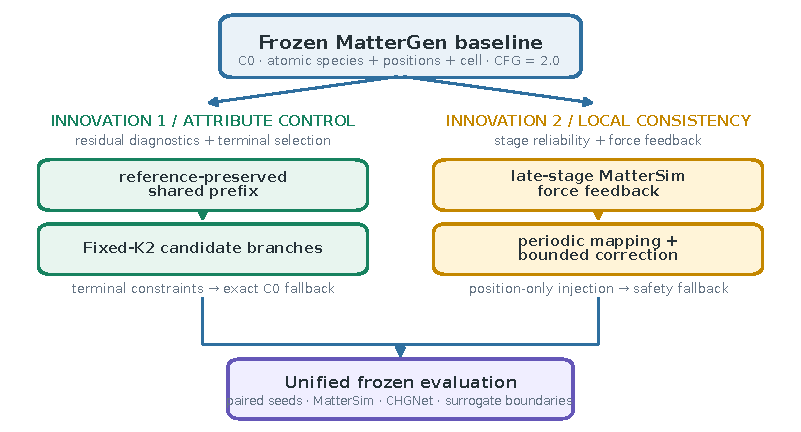
\includegraphics[keepaspectratio,alt={图1-1 本文总体技术路线}]{../../../thesis_release/concept_figures_polished/figure1_1_technical_route.pdf}}
\bicaption{本文总体技术路线}{Overall Technical Route of This Thesis}\label{fig:1-1}
\end{figure}

\section{论文组织结构}

第1章为绪论，介绍材料逆向生成的研究背景、代表性研究路线、现有问题、本文研究内容、两个创新点、技术路线和论文结构。

第2章为相关理论与关键技术，统一说明晶体的原子种类---周期分数坐标---晶胞表示、扩散生成、score和CFG，介绍MatterGen的三字段联合生成、GemNetT去噪网络、神经网络原子间势、Matter\allowbreak Sim和CHGNet，并定义后续章节使用的评价指标和配对统计方法。

第3章研究参考轨迹保留的预算约束多分支条件引导与安全回退方法。该章先分析在线Adaptive CFG和反事实候选空间，再介绍精确参考轨迹、共享前缀、Fixed-K2、终点约束和安全回退，并报告Fixed-K2的独立确认结果及Linear-K2负消融。

第4章研究基于阶段可靠性校准的后期神经力场引导扩散方法RC-NFGD。该章介绍预测干净结构的阶段诊断、Matter\allowbreak Sim力计算、笛卡尔---分数坐标映射、position predictor注入、有界修正和安全回退，并通过P0、Formal\allowbreak 32、Formal256和CHGNet交叉代理评价检验方法。

第5章在统一的冻结证据体系下综合比较两项创新，讨论属性精度、代理局部结构一致性、计算代价、跨代理方向、负消融、POST竞争基线及联合兼容性，明确当前结论的适用范围和未解决问题。

第6章总结全文工作，归纳两个创新点的主要结论、代理评价和计算成本边界，并展望跨属性、跨模型、DFT/实验验证及经重新预注册的联合方法研究。

\section{本章小结}

本章从材料搜索空间和逆向设计需求出发，回顾了晶体生成模型、扩散生成、条件属性控制和神经网络原子间势的发展。现有工作已经能够处理周期晶体表示、组成或空间群条件以及面向性质的候选生成，但在冻结生成模型中如何以受控预算进行安全的推理时选择，以及如何在可靠后期把神经势力反馈接入周期扩散轨迹，仍具有明确的研究价值。

围绕这两个问题，本文以MatterGen为基础模型，分别提出参考轨迹保留的预算约束多分支条件引导与安全回退方法，以及RC-NFGD。前者面向代理属性控制，后者面向代理局部结构一致性；两者独立评价，联合协同不作结论。第2章将进一步介绍本文涉及的晶体表示、扩散生成、条件引导和神经网络原子间势等理论基础。
